\documentclass[a4paper,12pt]{article} % тип документа

% Поля страниц
\usepackage[left=2.5cm,right=2.5cm,
    top=2cm,bottom=2cm,bindingoffset=0cm]{geometry}
    
%Пакет дял таблиц   
\usepackage{multirow} 
    
%Отступ после заголовка    
\usepackage{indentfirst}


% Рисунки
\usepackage{floatrow,graphicx,calc}
\usepackage{wrapfig}

%%% Работа с картинками
\usepackage{graphicx}  % Для вставки рисунков
\graphicspath{{images/}{images2/}}  % папки с картинками
\setlength\fboxsep{3pt} % Отступ рамки \fbox{} от рисунка
\setlength\fboxrule{1pt} % Толщина линий рамки \fbox{}
\usepackage{wrapfig} % Обтекание рисунков и таблиц текстом

% Создаёем новый разделитель
\DeclareFloatSeparators{mysep}{\hspace{1cm}}

% Ссылки?
\usepackage{hyperref}
\usepackage[rgb]{xcolor}
\hypersetup{				% Гиперссылки
    colorlinks=true,       	% false: ссылки в рамках
	urlcolor=blue          % на URL
}


%  Русский язык
\usepackage[T2A]{fontenc}			% кодировка
\usepackage[utf8]{inputenc}			% кодировка исходного текста
\usepackage[english,russian]{babel}	% локализация и переносы




% Математика
\usepackage{amsmath,amsfonts,amssymb,amsthm,mathtools}

%%% Дополнительная работа с математикой
\usepackage{amsmath,amsfonts,amssymb,amsthm,mathtools} % AMS
\usepackage{icomma} % "Умная" запятая: $0,2$ --- число, $0, 2$ --- перечисление


% Что-то 
\usepackage{wasysym}


\begin{document}
\begin{center}
	\footnotesize{ФЕДЕРАЛЬНОЕ ГОСУДАРСТВЕННОЕ АВТОНОМНОЕ ОБРАЗОВАТЕЛЬНОЕ 			УЧРЕЖДЕНИЕ ВЫСШЕГО ОБРАЗОВАНИЯ}\\
	\footnotesize{МОСКОВСКИЙ ФИЗИКО-ТЕХНИЧЕСКИЙ ИНСТИТУТ\\(НАЦИОНАЛЬНЫЙ 			ИССЛЕДОВАТЕЛЬСКИЙ УНИВЕРСИТЕТ)}\\
	\footnotesize{ФАКУЛЬТЕТ ОБЩЕЙ И ПРИКЛАДНОЙ ФИЗИКИ\\}
	\hfill \break
	\hfill \break
	\hfill \break
	\hfill \break
\end{center}


\begin{figure*}[h]
    \centering
    \includegraphics*[width=10cm,height=7cm,keepaspectratio]{mipt_eng_text_png.png}
    \label{fig:my_label}
\end{figure*}


\begin{center}   
    \hfill \break
	\hfill \break
	\hfill \break
	\large{Лабораторная работа № 4.3.2\\ \hfill \break\Large{Дифракция света на ультразвуковой волне в жидкости}}\\
	\hfill \break
	\hfill \break
	\hfill \break
	\hfill \break
	\begin{flushright}
		Баранов Даниил\\
		Группа Б02-103
	\end{flushright}
	\hfill \break
	\hfill \break
	\hfill \break
\end{center}
\hfill \break
\hfill \break
\hfill \break
\hfill \break
\begin{center}
	Долгопрудный, 2023 г.
\end{center}
\thispagestyle{empty}

\newpage


\textbf{Цель:} изучение дифракции света на синусоидальной акустической решётке и наблюдение фазовой решётки методом тёмного
поля.

\textbf{Используются в работе:} оптическая скамья, осветитель, два длиннофокусных объектива, кювета с жидкостью, кварцевый излучатель
с микрометрическим винтом, генератор ультразвуковой частоты, линза, вертикальная нить на рейтере, микроскоп.

\section{Теоретическая справка}
При прохождении ультразвуковой волны через жидкость в ней возникают периодические неоднородности коэффициента преломления, создается фазовая решетка, которую мы считаем неподвижной ввиду малости скорости звука относительно скорости света. Показатель
	преломления n изменяется по закону:
	
	\begin{equation}\label{}
	n = n_0 (1 + m \cos \Omega x)
	\end{equation}
	
	Здесь $ \Omega = 2 \pi / \Lambda $ --- волновое число для ультразвуковой волны, $ m $ --- глубина модуляции $ n $ $ (m \ll 1 $).
	
	Положим фазу $ \phi $ колебаний световой волны на передней стенке кюветы равной нулю, тогда на задней поверхности она равна:
	
	\begin{equation}\label{}
	\phi  = k n L = \phi_0 (1 + m \cos \Omega x)
	\end{equation}
	
	Здесь $ L $ --- толщина жидкости в кювете, $ k = 2 \pi / \lambda $ --- волновое число для света.
	
	После прохождения через кювету световое поле есть совокупность плоских волн, распространяющихся под углами $ \theta $, соответствующими максимумам в дифракции Фраунгофера:
	
\begin{equation}\label{}	
	\Lambda \sin \theta_m = m \lambda
\end{equation}

Этот эффект проиллюстрирован на рисунке 1.

	Зная положение дифракционных максимумов, по формуле (1) легко определить длину ультразвуковой волны, учитывая малость $ \theta $: $ \sin \theta \approx \theta \approx l_m /F  $, где $ l_m $ --- расстояние от нулевого до последнего видимого максимума, $ F $ --- фокусное расстояние линзы. Тогда получим:
	
	\begin{equation}\label{}
	 \Lambda = m \lambda F/ l_m 
	\end{equation}
	Скорость ультразвуковых волн в жидкости, где $ \nu $ --- частота колебаний излучателя:
	
\begin{equation}\label{}
	v = \Lambda \nu 
\end{equation}

\begin{figure}[H]
	\center{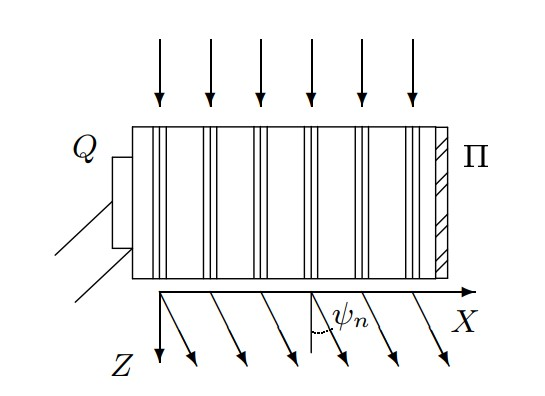
\includegraphics[scale=0.9]{1.jpg}}
  \caption{Эффект дифракции на ультразвуковой волне}
	\label{fig:image1}
\end{figure}

\section{Экспериментальная установка}
На рисунке 2 изображена схема экспериментальной установки. Источник света Л с помощью конденсора К проецируется на входную щель $S$. Входная щель ориентирована горизонтально и прикрыта красным светофильтром Ф. Коллиматорный объектив $\text{О}_1$ посылает параллельный пучок на кювету с водой $С$. Излучатель Q создаёт УЗ-волну. Параллельный пучок света, дифграгируя на стоячей звуковой волне, образует дифракционную картину в фокальной плоскости $F$ камерного объектива $\text{О}_{2}$. Картину можно наблюдать в микроскоп М.
\begin{figure}[H]
	\center{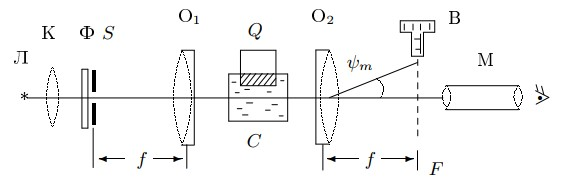
\includegraphics[scale=1]{2.jpg}}
  \caption{Схема экспериментальной установки}
	\label{fig:image1}
\end{figure}
\section{Ход работы}
\subsection{Определение скорости звука по дифракционной картине}
Изначально была собрана схема и проведена юстировка системы. Для различных частот генератора $Q$ изучаем дифракционную картину. Результаты измерений приведены в таблицах 1 и 2. Сами измерения производились в делениях, одно деление соответствует 4 микрометрам. Абсолютную погрешность считаем равной 1 делению.
\floatsetup[table]{capposition=top}

\begin{table}[H]
\begin{tabular}{|ll|ll|ll|}
\hline
\multicolumn{2}{|l|}{$\nu = 1,0084$ МГц} & \multicolumn{2}{c|}{$\nu = 1,17667 $ МГц} & \multicolumn{2}{l|}{$\nu = 1,51635$ МГц} \\ \hline
\multicolumn{1}{|l|}{m}   & $x_{m}$, мкм & \multicolumn{1}{l|}{m}    & $x_{m}$, мкм  & \multicolumn{1}{l|}{m}   & $x_{m}$, мкм  \\ \hline
\multicolumn{1}{|l|}{-4}  & 1036         & \multicolumn{1}{l|}{-4}   &               & \multicolumn{1}{l|}{-4}  &               \\ \hline
\multicolumn{1}{|l|}{-3}  & 912          & \multicolumn{1}{l|}{-3}   &               & \multicolumn{1}{l|}{-3}  &               \\ \hline
\multicolumn{1}{|l|}{-2}  & 788          & \multicolumn{1}{l|}{-2}   & 904           & \multicolumn{1}{l|}{-2}  & 988           \\ \hline
\multicolumn{1}{|l|}{-1}  & 660          & \multicolumn{1}{l|}{-1}   & 768           & \multicolumn{1}{l|}{-1}  & 836           \\ \hline
\multicolumn{1}{|l|}{0}   & 524          & \multicolumn{1}{l|}{0}    & 616           & \multicolumn{1}{l|}{0}   & 632           \\ \hline
\multicolumn{1}{|l|}{1}   & 416          & \multicolumn{1}{l|}{1}    & 476           & \multicolumn{1}{l|}{1}   & 444           \\ \hline
\multicolumn{1}{|l|}{2}   & 292          & \multicolumn{1}{l|}{2}    & 328           & \multicolumn{1}{l|}{2}   & 256           \\ \hline
\multicolumn{1}{|l|}{3}   & 176          & \multicolumn{1}{l|}{3}    &               & \multicolumn{1}{l|}{3}   &               \\ \hline
\multicolumn{1}{|l|}{4}   & 64           & \multicolumn{1}{l|}{4}    &               & \multicolumn{1}{l|}{4}   &               \\ \hline
\end{tabular}
\caption{Первая таблица первого пункта}
\end{table}
\begin{table}[h]
\begin{tabular}{|ll|ll|}
\hline
\multicolumn{2}{|l|}{$\nu = 1,9986$ МГц} & \multicolumn{2}{c|}{$\nu = 4,43 $ МГц} \\ \hline
\multicolumn{1}{|l|}{m}    & $x_{m}$, мкм   & \multicolumn{1}{l|}{m}    & $x_{m}$, мкм  \\ \hline
\multicolumn{1}{|l|}{-2}   & 960         & \multicolumn{1}{l|}{-2}   &            \\ \hline
\multicolumn{1}{|l|}{-1}   & 796         & \multicolumn{1}{l|}{-1}   & 1076       \\ \hline
\multicolumn{1}{|l|}{0}    & 508         & \multicolumn{1}{l|}{0}    & 560        \\ \hline
\multicolumn{1}{|l|}{1}    & 288         & \multicolumn{1}{l|}{1}    & 16         \\ \hline
\multicolumn{1}{|l|}{2}    & 40          & \multicolumn{1}{l|}{2}    &            \\ \hline
\end{tabular}
\caption{Вторая таблица первого пункта}
\end{table}
\\
По наклонам графиков определяем длину волны для каждой частоты по формуле 4 и скорость звука по формуле 5. Результаты приведены в таблице 3.
\\
\begin{figure}[H]
	\center{\includegraphics[scale=0.9]{plot7.eps}}
  \caption{\centering График зависимости $x_{m}$ от m для частоты 1,0084 МГц. Наклон кривой $k = -122,3 \pm 1,1$ мкм
}
	\label{fig:image1}
\end{figure}
\begin{figure}[H]
	\center{\includegraphics[scale=0.9]{plot6.eps}}
  \caption{\centering График зависимости $x_{m}$ от m для частоты 1,17667 МГц. Наклон кривой $k = -144 \pm 2$ мкм
}
	\label{fig:image1}
\end{figure}
\begin{figure}[H]
	\center{\includegraphics[scale=0.9]{plot5.eps}}
  \caption{\centering График зависимости $x_{m}$ от m для частоты 1,51635 МГц. Наклон кривой $k = -185 \pm 2$ мкм
}
	\label{fig:image1}
\end{figure}
\begin{figure}[H]
	\center{\includegraphics[scale=0.9]{plot4.eps}}
  \caption{\centering График зависимости $x_{m}$ от m для частоты 1,9986 МГц. Наклон кривой $k = -234 \pm 4$ мкм
}
	\label{fig:image1}
\end{figure}
\begin{figure}[H]
	\center{\includegraphics[scale=0.9]{plot3.eps}}
  \caption{\centering График зависимости $x_{m}$ от m для частоты 4,43 МГц. Наклон кривой $k = -530 \pm 8$ мкм
}
	\label{fig:image1}
\end{figure}
\begin{table}[H]
\begin{tabular}{|l|l|l|}
\hline
$\nu$, МГц & $\Lambda$, м & c    \\ \hline
1,0084     & 0,001465     & 1478 \\ \hline
1,17667    & 0,001244     & 1464 \\ \hline
1,51635    & 0,000969     & 1469 \\ \hline
1,9986     & 0,000766     & 1531 \\ \hline
4,43       & 0,000338     & 1498 \\ \hline
\end{tabular}
\caption{\centering Таблица со значениями длин волн и скоростей,\\ посчитанными для разных частот}
\end{table}
Основную часть относительной погрешности измерения скорости звука составляет погрешность, возникающая из-за того, что фильтр пропускает диапазон частот, суммарная погрешность не превышает 3,5 процентов. Средняя скорость по результатам всех измерений равна $c = 1490\pm 50$ м/c, что согласуется с табличным значением $c = 1490$ м/c.
\subsection{Определение скорости звука методом тёмного поля}
В данном пункте скорость ультразвука измеряется методом тёмного поля, для этого между микроскопом и щелью размещается дополнительная линза. Откалибруем схему, определим цену деления окулярной шкалы 1 дел = 1,25 мм.
\\
Меняя частоту, будем наблюдать акустическую решётку. С помощью окулярной шкалы измерим при каждой частоте координаты первой и последней тёмной полосы, а также количество светлых промежутков между ними. Результаты измерений приведены в таблице 4. По данным также расчитаны длины УЗ-волн при разных частотах (с учётом удвоения числа наблюдаемых полос).
\begin{table}[H]
\begin{tabular}{|l|l|l|l|l|l|}
\hline
$\nu$, МГц & $x_{1}$, дел & $x_{n}$, дел & n-1 & $\Lambda $, мм & $\varepsilon_{\Lambda}$ \\ \hline
1,27241                 & 0,35         & 5            & 10  & 1,163          & 0,022                  \\ \hline
2,13342                 & 0,5          & 5,1          & 17  & 0,676          & 0,022                  \\ \hline
1,13638                 & 0,5          & 6,1          & 11  & 1,273          & 0,018                  \\ \hline
1,06176                 & 0,15         & 6,15         & 11  & 1,364          & 0,017                  \\ \hline
1,52526                 & 0,1          & 5,2          & 13  & 0,981          & 0,020                  \\ \hline
1,76265                 & 0            & 5,5          & 16  & 0,859          & 0,018                  \\ \hline
\end{tabular}
\caption{Таблица с измерениями методом тёмного поля}
\end{table}
\\
\begin{figure}[H]
	\center{\includegraphics[scale=0.9]{plot2.eps}}
  \caption{\centering График зависимости длины волны от обратной частоты
}
	\label{fig:image1}
\end{figure}
По таблице построен график зависимости длины волны от обратной частоты. Угловой коэффициент наклона равен $c = 1415 \pm 80$ м/c. Значение получилось сильно заниженным из-за большой погрешности измерений, но, в целом, сходится с тем, что получилось в предыдущем пункте. 
\section{Вывод}
В данной работе была исследована дифракция света на ультразвуковой волне в жидкости. С помощью измерений была определена скорость ультразвука (двумя способами - непосредственно по дифракционной картине и методом тёмного поля). Первый способ позволил достаточно точно определить скорость звука, полученное значение хорошо сошлось с табличным, во втором способе значение получено менее точно из-за больших погрешностей при измерений координат полос, однако всё же сходится с табличным. 


\end{document}
